\documentclass[tikz,border=4pt]{standalone}
\usepackage[T1]{fontenc}\usepackage[utf8]{inputenc}\usepackage{helvet}\renewcommand{\familydefault}{\sfdefault}
\begin{document}
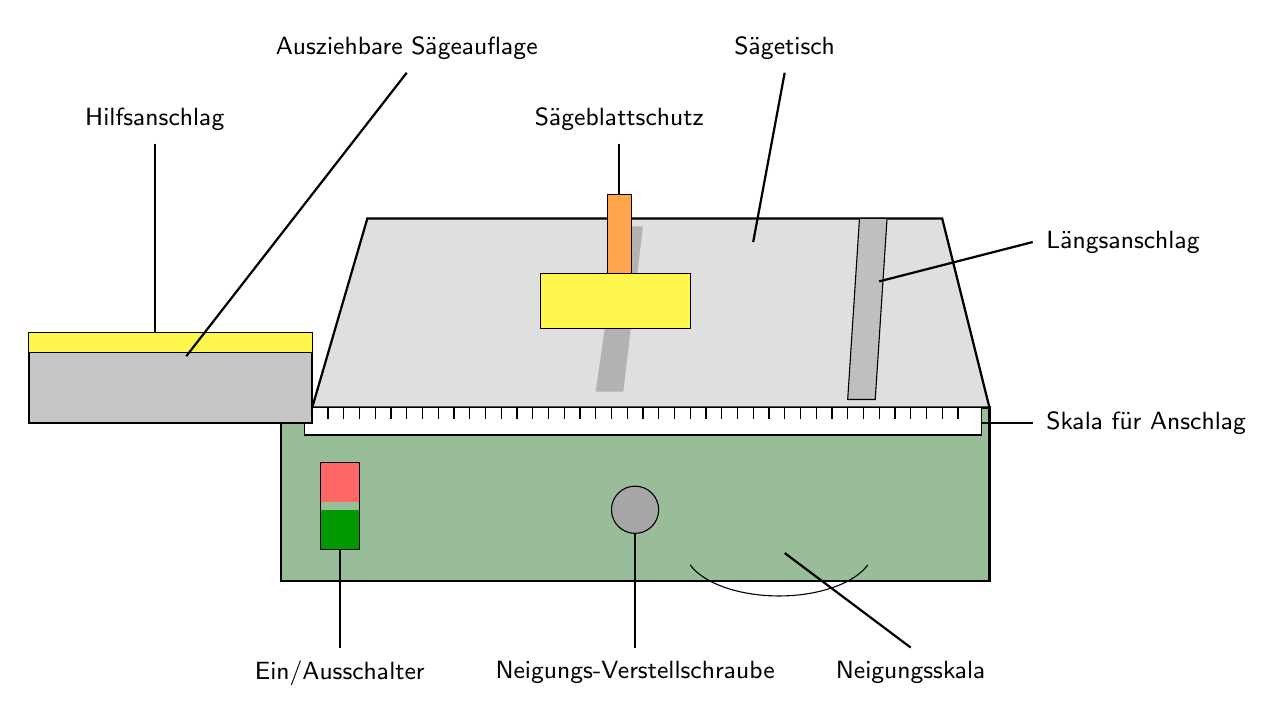
\begin{tikzpicture}[font=\small, lbl/.style={draw=black, thick}]
% Grundgehäuse (Vorderansicht unten, Draufsicht oben)
\fill[green!35!black!40] (0,0) rectangle (9,2.2);              % Gehäuse
\draw[thick] (0,0) rectangle (9,2.2);
\fill[gray!25] (0.4,2.2) -- (1.1,4.6) -- (8.4,4.6) -- (9,2.2) -- cycle; % Sägetisch
\draw[thick] (0.4,2.2) -- (1.1,4.6) -- (8.4,4.6) -- (9,2.2) -- cycle;
\fill[gray!60] (4.0,2.4) -- (4.3,4.5) -- (4.6,4.5) -- (4.35,2.4) -- cycle; % Schlitz
% Sägeblattschutz
\fill[yellow!70] (3.3,3.2) rectangle (5.2,3.9); \draw (3.3,3.2) rectangle (5.2,3.9);
\fill[orange!70] (4.15,3.9) rectangle (4.45,4.9); \draw (4.15,3.9) rectangle (4.45,4.9);
% Längsanschlag rechts
\fill[gray!50] (7.2,2.3) -- (7.35,4.6) -- (7.7,4.6) -- (7.55,2.3) -- cycle; \draw (7.2,2.3) -- (7.35,4.6) -- (7.7,4.6) -- (7.55,2.3) -- cycle;
% Skala
\fill[white] (0.3,1.85) rectangle (8.9,2.2); \draw (0.3,1.85) rectangle (8.9,2.2);
\foreach \x in {0.4,0.6,...,8.8}{\draw (\x,2.2) -- (\x,2.05);}
% ausziehbare Auflage links mit Hilfsanschlag
\fill[gray!45] (-3.2,2.0) rectangle (0.4,2.9); \draw[thick] (-3.2,2.0) rectangle (0.4,2.9);
\fill[yellow!70] (-3.2,2.9) rectangle (0.4,3.15); \draw (-3.2,2.9) rectangle (0.4,3.15);
% Schalter, Neigungsschraube, Skala
\fill[red!60] (0.5,1.0) rectangle (1.0,1.5); \fill[green!60!black] (0.5,0.4) rectangle (1.0,0.9); \draw (0.5,0.4) rectangle (1.0,1.5);
\fill[gray!70] (4.5,0.9) circle (0.3); \draw (4.5,0.9) circle (0.3);
\draw (5.2,0.2) arc[start angle=200,end angle=340,x radius=1.2cm,y radius=0.6cm];
% Beschriftungen
\node[above] at (-1.6,5.6) {Hilfsanschlag}; \draw[lbl] (-1.6,5.55) -- (-1.6,3.15);
\node[above] at (1.6,6.5) {Ausziehbare Sägeauflage}; \draw[lbl] (1.6,6.45) -- (-1.2,2.85);
\node[above] at (4.3,5.6) {Sägeblattschutz}; \draw[lbl] (4.3,5.55) -- (4.3,4.9);
\node[above] at (6.4,6.5) {Sägetisch}; \draw[lbl] (6.4,6.45) -- (6.0,4.3);
\node[right] at (9.6,4.3) {Längsanschlag}; \draw[lbl] (9.55,4.3) -- (7.6,3.8);
\node[right] at (9.6,2.0) {Skala für Anschlag}; \draw[lbl] (9.55,2.0) -- (8.9,2.0);
\node[below] at (0.75,-0.9) {Ein/Ausschalter}; \draw[lbl] (0.75,-0.85) -- (0.75,0.4);
\node[below] at (4.5,-0.9) {Neigungs-Verstellschraube}; \draw[lbl] (4.5,-0.85) -- (4.5,0.6);
\node[below] at (8.0,-0.9) {Neigungsskala}; \draw[lbl] (8.0,-0.85) -- (6.4,0.35);
\end{tikzpicture}
\end{document}
